\section{Introduction}
\label{sec:alkbw:intro}

As discussed in Chapter~\ref{ch:dbb}, the LR6 Zn-MnO2 alkaline AA battery has been the mainstay of the primary battery market for nearly 60 years.~\cite{karl_patent} The low cost and abundance of the source materials have made alkaline AA batteries one of the most ubiquitous electrochemical energy storage cells, with over 40 million kgs sold in 2013 alone.~\cite{highbeam,ibisworld} Despite this ubiquity, there is still much to be learned about the materials properties of this system. Numerous studies have been performed \textit{ex situ} on Zn and \ce{MnO2} in alkaline solutions to understand the processes that occur at each electrode.\cite{arise,Balachandran2002-vd,Chen1993-bw,Chin1982-lw,Kozawa1966-ga,Kozawa1965-yt,Liu1981-ub,McLarnon1991-bw,Pandya1995-tg} In addition, \textit{ex situ} mechanical testing has shown that microscopic morphological changes in the Zn anode can affect a macroscopic change in the mechanical response of the full cell, as detailed in Chapter~\ref{ch:dbb}.~\cite{Bhadra2015-aq} Thus far, however, \textit{in operando} efforts have been limited to either neutron tomography,~\cite{Manke2007-yj,Riley2010-ur} or large scale experiments using synchrotron sources to perform EDXRD,~\cite{gallaway,Gallaway2015-xy} or x-ray microtomography.~\cite{haibel, Manke2007-yj}

In Chapter~\ref{ch:bw}, we demonstrated a technique which was applicable to most battery chemistries and provided in operando monitoring of both state of charge and state of health through non-destructive mechanical interrogation: EAToF.~\cite{Hsieh2015-kr} This method uses an ultrasonic contact transducer to generate an acoustic pulse. The resulting pulse will display different ToF profiles based on the sound speed of the battery component materials. Sound speed, \emph{c}, in a material scales with the bulk modulus, \emph{B}, and inversely with the density, \emph{$\rho$} as shown previously in Equation~\ref{eq:newtonlaplace}, and as both of these materials properties change as a function of state of charge and state of health we can use the ToF profiles to analyze the state of the battery.

\begin{equation*}
c= \sqrt{\frac{B}{\rho}}
\tag{\ref{eq:newtonlaplace}}
\end{equation*}

In this chapter, we applied EAToF measurements to LR6 alkaline AA batteries. The LR6 uses a unique bobbin geometry, detailed previously in Fig.~\ref{fig:aaschem}, in which each electrode occupies a large contiguous volume within the cell, unlike in jelly roll geometries where thin electrode layers are rolled to fill the cylindrical or prismatic volume. As a result, there are relatively few interfaces for scattering of the ultrasonic pulse and ample regions of each material through which the pulse can travel. In alkaline AA batteries, the relevant density and modulus shifts are strongest in the Zn anode due to a densification and dehydration of the initial Zn gel into a porous ZnO solid which occurs radially beginning at the separator and progressing inwards to the central current collecting pin.~\cite{Bhadra2015-aq} This transition results in a 39\% change in density and a 107\% change in bulk modulus based on the materials property information in Table 1. EAToF allows us to see this densification of the anode due to oxidation during discharge but also offers more insight into the quality of the anode materials, which we demonstrate by performing EAToF measurements on a number of brands of alkaline AA batteries. We show that cells displaying greater discharge capacity also have pronounced differences in the EAToF transmission profiles of their respective anodes.

\begin{figure}[htb]
  \centering
    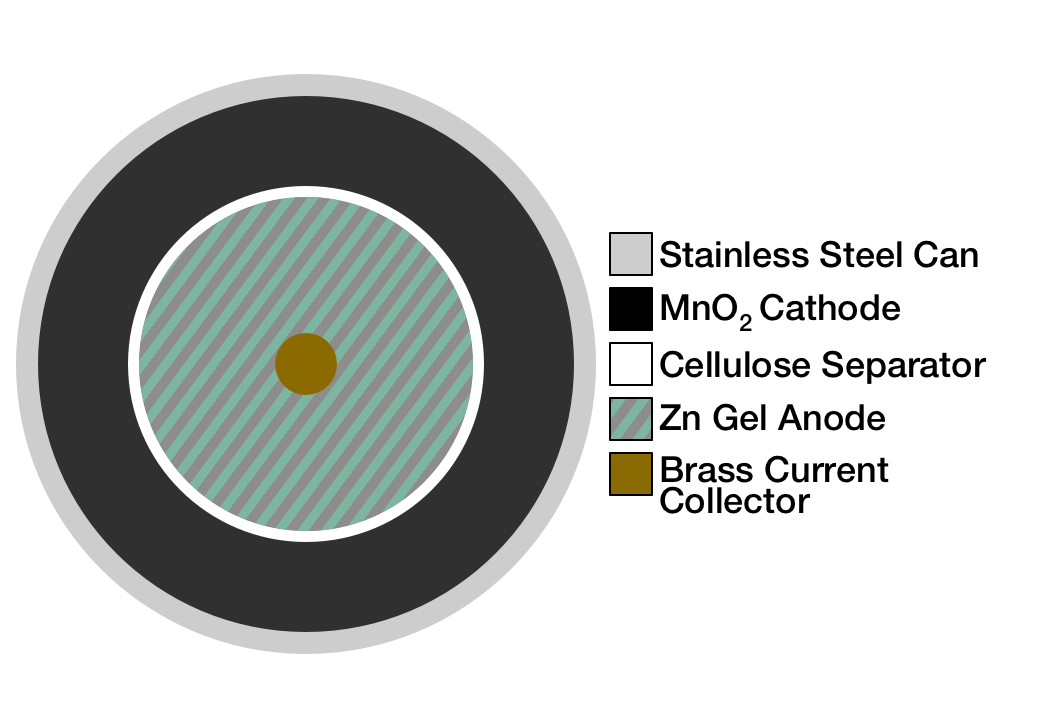
\includegraphics[width=0.80\textwidth]{ch3-dbb/Images/aaschem.png}
    \repeatcaption{fig:aaschem}{Schematic of construction of a alkaline AA battery. Components are labeled according to the legend.}
\end{figure}

\begin{table}[htb]
\centering
  \repeatcaptiont{tab:table3}{Materials properties of electrode materials in an alkaline battery}
  \begin{tabular}{*{4}{l}}
    \hline
    Material & Density (g/cm$^3$) & Bulk modulus (GPa) & Reference\\
    \hline
        Zinc (Zn)& 7.05 & 72.0 & ~\cite{Kaye2014-am}\\
        Zinc oxide (ZnO) & 5.06 & 134.0 & ~\cite{Munro2002-pg}\\
        Zn gel & 3.64 (est.) & 57.6 (est.) & ~\cite{Kaye2014-am,Murei2007-ke}\\
        Electrolytic (\ce{MnO2}) & 4.55 & 54.5 & ~\cite{Robert1990-zl,Tao2013-vg}\\
        Groutite (MnOOH) & 4.14 & 39.8 & ~\cite{Robert1990-zl,Tao2013-vg}\\
  \end{tabular}
\end{table}


